\documentclass[14pt]{article}
\usepackage[T2A]{fontenc} 
\usepackage[utf8]{inputenc}
\usepackage{alltt}
\usepackage[english,russian]{babel}
\usepackage{amsmath}
\usepackage{amsfonts}
\usepackage{amssymb}
\usepackage{wrapfig}
\usepackage{indentfirst}
\usepackage{setspace}
\usepackage[pdftex]{graphicx}
\usepackage{caption}
\usepackage{subcaption}
\usepackage{textcomp}
\usepackage{array}
\usepackage[T1]{fontenc}
\usepackage{librebaskerville}

\topmargin = -1.5cm
\marginparwidth = -1cm
\marginparsep = 0pt
\textwidth = 16cm
\textheight = 24cm
\oddsidemargin = 0.2cm
\parindent = 0.5cm
\lineskip = 0.025cm
\parskip = 0.2cm




\begin{document}

\begin{titlepage}

\newcommand{\HRule}{\rule{\linewidth}{0.5mm}} 
\centering 

\begin{figure}
    \centering
    \begin{subfigure}{1.5cm}
        
\includegraphics[height=1.3cm]{msu.jpg}
    \end{subfigure}
    \parbox[t][0.2cm][c]{12cm}{
        \centering
        \large Московский государственный университет имени М.~В.~Ломоносова\\[0.5cm]
        \normalsize Факультет вычислительной математики и кибернетики
    }
    \begin{subfigure}{1.25cm}    
        
\includegraphics[height=1.25cm]{cmc.jpg}
    \end{subfigure}
\end{figure}



\HRule \\[5cm]
{
 \bfseries \upshape
{ \Huge  \guillemotleftРекурсивные нейросети с памятью\guillemotright }\\[0.2cm]
{\LARGE Реферат}\\[0.2cm]

{
\large
\vspace{1cm}
студента $203$ учебной группы факультета ВМК МГУ \\
Щербакова Александра Станиславовича
}

\vspace{9cm}
{\large Москва, \today}
} 


\vfill

\end{titlepage}

\tableofcontents
\pagebreak
\section{Введение}

\large
Рекурсивные нейронные сети (Recursive Neural Networks, RNN) известны уже около 20-ти лет. Это вид глубоких нейронных сетей, которые работают с некоторым набором весов рекурсивно. Рекурсивные нейросети используются для обработки естественных языков, работы с последовательностями, изображениями.


\section{Рекурсивные нейросети}

\subsection{Описание}
\largeРекурсивные нейронные сети подходят для задачи классификации и регрессии. Они широко используются в моделях с информацией в числовом и символьном виде. Важным преимуществом рекурсивных нейросетей является их возможность работать с информацией имеющей топологию отличную от вектора фиксированного размера. Таким образом для информации, представленной в виде графа, сохраняются связи между вершинами графа. Но есть существенное ограничение на топологию графов, с которыми ведет работу нейронная сеть этого типа - они должны быть ацикличны. Это связано с тем, что ребра графа интерпретируются как причинно-следственная связь. Есть примеры рекурсивных нейронных сетей, которые обрабатывают циклические графы, но они, как правило, могут быть использованы только в очень редких конкретных видах задач.


Второе ограничение связано с достаточно слабым математическим аппаратом такой сети. В частности, отсутствие такой операции как сумма графов.


В качестве алгоритма для обучения рекурсивной нейронной сети можно использовать алгоритм стохастического градиентного спуска второго порядка. Этот метод устойчив к затуханию градиента. Так же он обеспечивает оптимальный компромисс между скоростью сходимости и вычислительносй сложностью вычислений.


Можно провести параллель между такой сетью и интеллектом. У интеллекта есть два основопологающий принципа: максимизация передачи и принцип возвратности. Первый из них гласит, что всегда, когда это возможно интеллектуальная система накапливает знания путем максимизации передачи полученных ранее знаний. Таким образом система становится более сложной накапливая все новые знания. Принцип возвратности связывает память и логические выводы. Он утверждает, что система является интеллектуальной, если она может восстановить причины своего состояния.

\subsection{Структура}
\largeПусть дан граф $U = (V, E)$. Для вершины $v\in V$ $pa[v]$ - множество вершин родителей, $ch[v]$ - множество  дочерних вершин. Под родительской вершиной будем подразумевать ту, в которую ведет ребро из $v$, а под дочерней - вершину, из которой есть ребро в $v$. Этот граф будет описывать единицы информации, с которыми работает нейросеть. В каждой вершине содержится фрагмент информации, а налачие ребра между двумя вершинами подразумевает их связь.


Модель рекурсивной нейронной сети включает в себя функцию изменения состояния $f$ и выходную функцию $g$. Обычно эти функции реализуются многослойным перцептроном. Стандартная модель подходит для обработки направленных ациклических графов с одним корнем. Они реализуют пересчет состояния сети с учетом предыдущего шага:


\begin{eqnarray}
&a(v) = f(a(ch[v]), I(v), v, W_f)\nonumber\\
&y(v) = g(a(v), v, W_g)
\end{eqnarray}


Где $W_f$ и $W_g$ - матрицы синаптических весов для сетей $f$ и $g$. Это параметры модели. $a(v)$ - состояние вершины. Для каждой вершины состояние пересчитывается из входного сигнала $I(v)$ и состояний дочерних вершин $ch[v]$.


\begin{equation}
\label{trivial}
a(ch[v]) = [a(ch_1[v]), a(ch_2[v]), \dots, a(ch_o[v])]
\end{equation}


В выражении $(2)$ $o$ - максимальное количество дочерних элементов. Результат работы нейронной сети (вывод вершины-корня $s$) вычисляется по формуле $y = g(a(s))$.


\begin{figure}[!h]
    \centering
        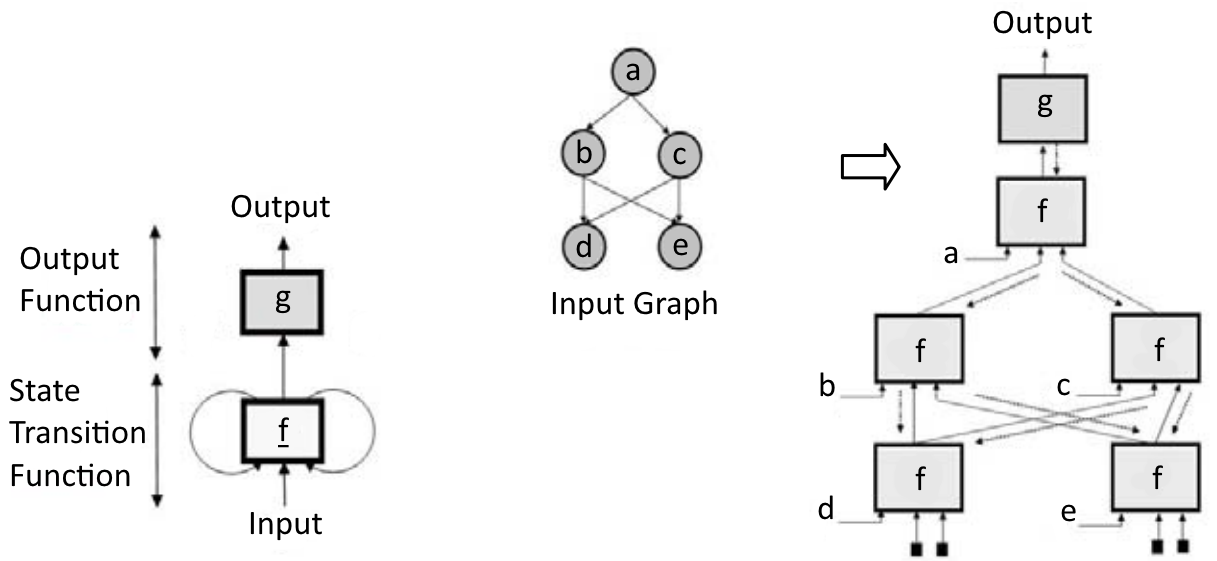
\includegraphics[height=7cm]{Fig1.png}
    \parbox[t][1.2cm][c]{16cm}{
        \centering
        Рис. 1. Пример входного графа и рекурсивной  нейронной сети
    }
\end{figure}


\subsection{Обучение}
Алгоритмы обучения нейронных сетей строятся на минимизации некоторой функции $E(W)$ - функции ошибки. Соответственно, изменяется ее параметр $W$.


В случае рекурсивных нейронных сетей фаза обучения состоит из подбора параметров функции изменения состояния $f$ и выходной функции $g$. Обозначим вектор параметров этих функций через $W = [w_1, w_2, \dots, w_m]$. Тогда возмущение функции ошибки относительно некоторой точки можно записать в виде\\ $E(W + \Delta W) = E(w_1 + \Delta w_1, w_2 + \Delta w_2, \dots, w_m + \Delta w_m)$. Воспользуемся разложением в ряд Тейлора этой функции:


\begin{multline}
\label{trivial}
E(W + \Delta W) = E(W) + \sum\limits_{i = 1}^m\frac{\partial E(W)}{\partial w_i}\Delta w_i +
\frac{1}{2}\sum\limits_{i = 1}^m\frac{\partial^2 E(W)}{\partial w_i^2}(\Delta w_i)^2 +\\
+\sum\limits_{i < j}\frac{\partial^2 E(W)}{\partial w_i \partial w_j}\Delta w_i \Delta w_j+
\frac{1}{6}\sum\limits_{i = 1}^m\frac{\partial^3 E(W)}{\partial w_i^3}(\Delta w_i)^3 + \dots
\end{multline}


Итак, каждое обновление параметров модели (весов) можно рассматривать как возмущение относительно некоторой точки, заданное $m$-мерным вектором. Пусть задана послудевательность из $N$ таких векторов с возмущением $\Delta W^i, i = \overline{1, N}$. В формуле $(3)$ отбросим все члены третьего и более высоких порядков и выразим математическое ожидание функции ошибки:


\begin{multline}
\label{trivial}
\mathbb{E}(E(W)) = \frac{1}{N}\sum\limits_{n = 1}^N E(W + \Delta W^n)\\
\mathbb{E}(E(W)) = E(W) + \sum\limits_{i = 1}^m\frac{\partial E(W)}{\partial w_i}\frac{1}{N}\sum\limits_{n=1}^N\Delta w_i^n+ \frac{1}{2}\sum\limits_{i=1}^m\frac{\partial^2E(W)}{\partial w_i^2}\frac{1}{N}\sum\limits_{n=1}^N(\Delta w_i^n)^2 
+\\+\sum\limits_{i<j}\frac{\partial^2E(W)}{\partial w_i\partial w_j}\frac{1}{N}\sum\limits_{n=1}{N}\Delta w_i^n\Delta w_j^n
\end{multline}


Перепишем равенство $(4)$ в терминах моментов случайных величин:


\begin{multline}
\mathbb{E}(E(W)) \cong E(W) + \sum\limits_{i=1}^m\mathbb{E}(\Delta w_i)\frac{\partial E(W)}{\partial w_i} +
\frac{1}{2}\sum\limits_{i=1}^{m}\mathbb{D}(\Delta w_i)\frac{\partial^2E(W)}{\partial w_i^2} +\\
+ \sum\limits_{i<j}cov(\Delta w_i, \Delta w_j)\frac{\partial^2E(W)}{\partial w_i \partial w_j}
\end{multline}


Так как обучение проводится методом градиентного спуска, то $\Delta w_i = -\eta g_i$.  Слагаемым, содержащим $cov(\Delta w_i, \Delta w_j)$, можно принебречь в предположении, что возмущенния не коррелируют в зависимости от $n$. $\mathbb{E}(\Delta w_i)\approx 0$, поэтому можно отбросить первую сумму в $(5)$. $\mathbb{D}(\Delta w_i)$ перепишем в виде $\sigma^2(\Delta w_i)$. В итоге получим:


\begin{equation}
\mathbb{E}(E(W)) \cong E(W) +
\frac{1}{2}\sum\limits_{i=1}^{m}\sigma^2(\Delta w_i)\frac{\partial^2E(W)}{\partial w_i^2} = E(W) + \frac{\eta^2}{2}\sum\limits_{i=1}^{m}\sigma^2(g_i)\frac{\partial^2E(W)}{\partial w_i^2}
\end{equation}


Видно, что значение ошибки достаточно сильно зависит от $\Delta w_i$. Поэтому, чтобы подавить возможный шум $\Delta w_i$ может быть заменено на $\eta g_i / \sigma(g_i)$. Заметим, что таким образом сигнал ошибки становится меньше, но в то же время меньше становится и объем информации, которую накапливает сеть. Это известная проблема, которая затрудняет поддержку долговременных связей. В случае рекурсивных нейросетей это становится особенно критично. Но с другой стороны, это позволяет избежать затухание градиента.


Таким образом обучение рекурсивной нейронной сети производится градиентным спуском второго порядка.
\section{\hugeРекурентные нейросети}

\subsection{\LARGEОписание}

\subsection{\LARGEСтруктура}

\subsection{\LARGEОбучение}


\section{\huge LSTM}

\subsection{\LARGEОписание}

\subsection{\LARGEСтруктура}

\subsection{\LARGEОбучение}


\section{\hugeПримеры использования рекурсивных сетей}

\subsection{\LARGEОбработка естественных языков}

\subsection{\LARGEОбработка изображений}


\section{\hugeЗаключение}

\end{document}
